\documentclass[aspectratio=169,usenames,dvipsnames]{beamer}
\beamertemplatenavigationsymbolsempty
% \documentclass{beamer}

% UNCOMMENT FOR HANDOUTS
% \usepackage{pgfpages}
% \pgfpagesuselayout{2 on 1}[landscape,letterpaper,border shrink=5mm]
% \setbeameroption{show notes}

\mode<presentation>
\usetheme{Boadilla}
\usecolortheme{spruce}
\usepackage{../../LizStyle,ulem}
\usepackage{color}
\usepackage[color,matrix,arrow]{xy}


% \input xy
% \xyoption{all}
\usepackage{tikz}
\usepackage{tikz-cd}

\tikzset{commutative diagrams/diagrams={ampersand replacement=\&}}

\AtBeginSection{\frame{\sectionpage}}


% ==========Command for putting comments and removing them=======
% Visible:
\newcommand{\InstructorNotes}[1]{\textit{\color{orange}#1}}
\newcommand{\InstructorList}[1]{
\begin{itemize}
	\color{orange}
	#1
\end{itemize}
}
% Removed:
% \renewcommand{\InstructorNotes}[1]{} 
% \renewcommand{\InstructorList}[1]{}


\newcommand{\bvfill}{\vskip0pt plus 1filll}

\usepackage{multimedia}
\usepackage{graphbox}

% \usepackage{algpseudocode}


\newcommand{\Reeb}{\textbf{Reeb}}
\newcommand{\Rtopc}{\textbf{Rtopc}}
% \newcommand{\RR}{\mathcal{R}}

\newcommand{\Set}{\textbf{Set}}
\newcommand{\Vect}{\textbf{Vect}}
\newcommand{\Top}{\textbf{Top}}
\newcommand{\Int}{\textbf{Int}}

\graphicspath{ {Figures/} {../Figures/}{../../Figures/} }

\begin{document}
%\pdfoptionpdfminorversion 5
%\logo{\includegraphics[height=1.5cm]{dukeshield.pdf}}
\title[]{Ch 5.1.1-2: Leave One Out Cross-validation}
\subtitle{Lecture 12 - CMSE 381}
\date{Fri, 2/13, 2026}



\institute[MSU-CMSE]{Michigan State University\\
			::\\
          Dept of Computational Mathematics, Science \& Engineering}


\begin{frame}
 \titlepage


\end{frame}
%--------------------------
\begin{frame}[t]{Announcements }

\begin{columns}
\column{.45\textwidth}
\centering

	\textbf{Last time:}
	\begin{itemize}
		\item Exam
	\end{itemize}
	\textbf{Announcements:}
	\begin{itemize}
		\item Exam 1 grades.... hopefully soon
		% \item HW \#4 will be posted later next week. 
		% \item Drops 
		% \item Grade conversion 
		% 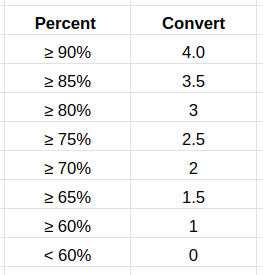
\includegraphics[align = c, width = .5\textwidth]{GradeConversion}
		
	\end{itemize}
\column{.45\textwidth}
\centering
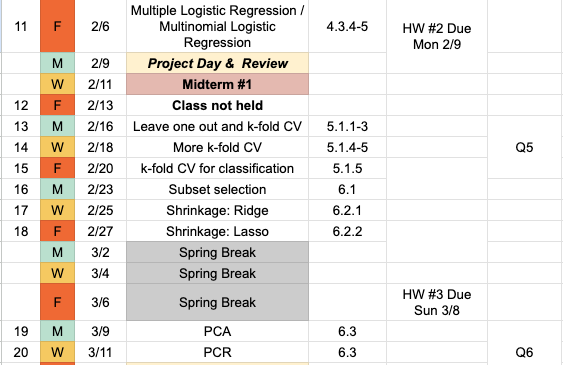
\includegraphics[width=\textwidth]{Schedule-S26-Lecs11_to_20}

\end{columns}

\end{frame}
%--- Next Frame ---%
\begin{frame}[c]{Covered in this lecture }

\begin{columns}
\column{.4\textwidth}
\centering
\begin{itemize}
	\item Validation Set
	\item LOO CV

\end{itemize}

\column{.4\textwidth}
\centering
\InstructorList{
  \item Previous versions of the course with more time I talked about the special case with linear regression. Due to time constraints, the slides below are commented out: 
	\item Outliers
	\item Leverage statistic
}

\end{columns}

\end{frame}
%--- Next Frame ---%


%=================
\section{Validation set}
%=================
\begin{frame}[c]{What's the problem?}

\begin{columns}
\column{6\textwidth}
\centering
\begin{itemize}
	\item How well is my ML method doing? \textit{Model Assessment}
	\item Which method is best for our data?
	\item How many features should I use? Which ones? \textit{Model selection}
	\item What is the uncertainty in the learned parameters?
\end{itemize}

\end{columns}
\InstructorNotes{First, Cross Validation. Then Bootstrap.}
\end{frame}
%--- Next Frame ---%
\begin{frame}[t]{Training Error vs Testing Error}

\begin{columns}
\column{.45\textwidth}
\centering
\textbf{Training Error}

\InstructorNotes{Easily calculated by applying stats learning method to the observations used in its training}

\InstructorList{
\item Massive under estimate
\item overfitting!
}

\column{.45\textwidth}
\centering
\textbf{Testing Error}

\InstructorNotes{Avg error that results from using a statistical learning method to predict the response on a new observation, one that was not used in training the method.}

\end{columns}

\end{frame}
%--- Next Frame ---%
\begin{frame}[c]{Throw-back}

	\centering
	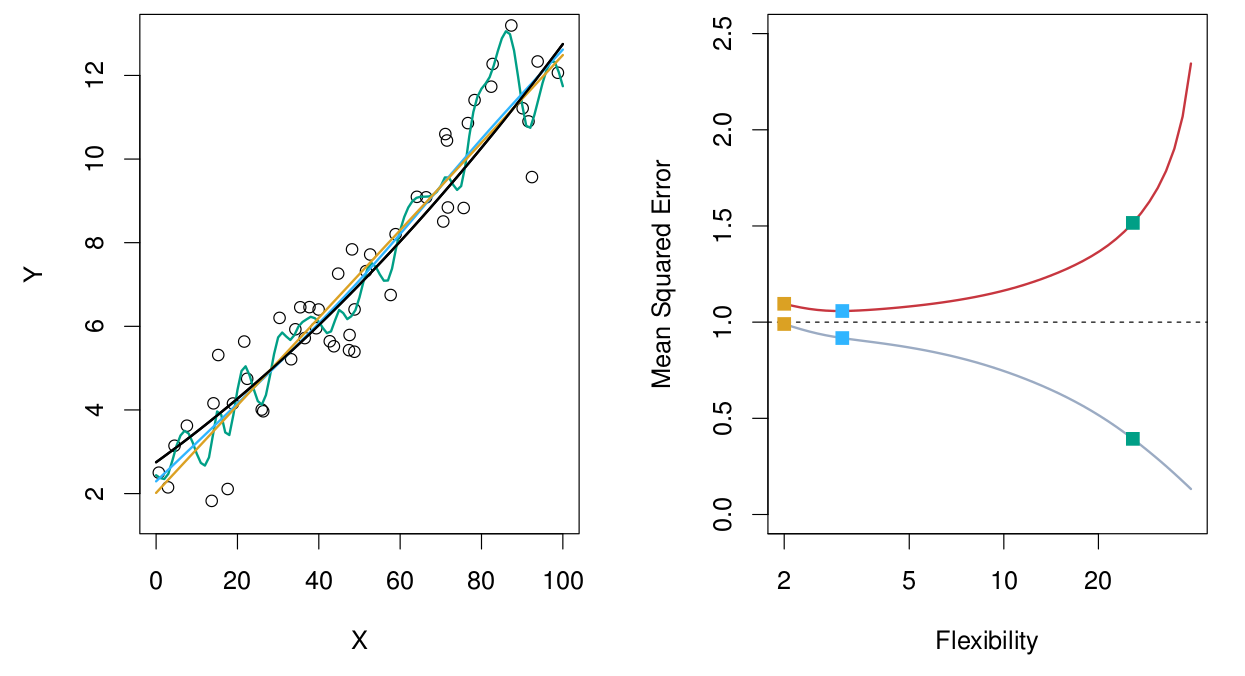
\includegraphics[width = .8\textwidth]{Fig2-10}
	

	\InstructorNotes{Grey is training error, red is testing error}
\begin{columns}
\column{.45\textwidth}
\centering

\column{.45\textwidth}
\centering

\end{columns}

\end{frame}
%--- Next Frame ---%
\begin{frame}[c]{Model tradeoffs}
\centering
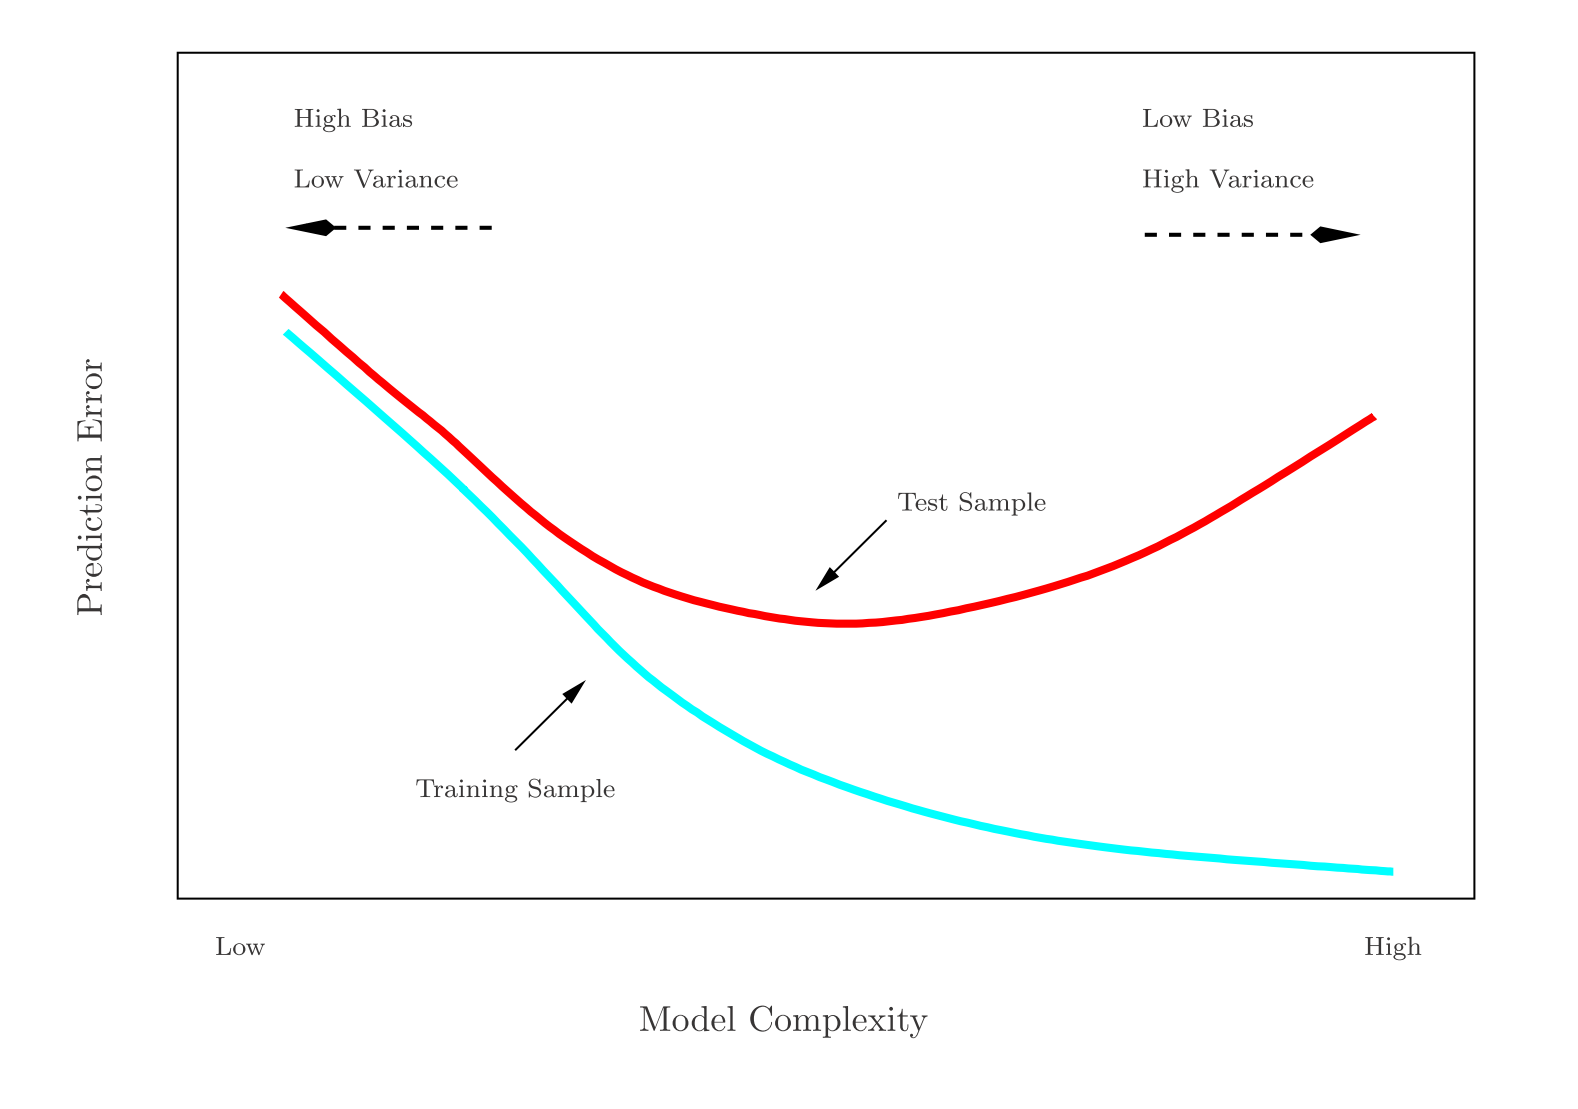
\includegraphics[width = .7\textwidth]{ModelTradeoffs.png}
\begin{columns}
\column{.45\textwidth}
\centering

\column{.45\textwidth}
\centering

\end{columns}

\end{frame}
%--- Next Frame ---%
\begin{frame}[t]{Validation set approach}

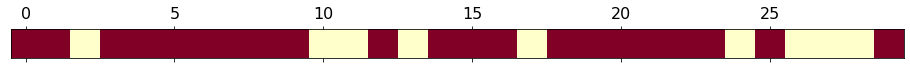
\includegraphics[width = \textwidth]{CV-subset0}

\begin{columns}
\column{.45\textwidth}
\centering
\begin{itemize}
	\item Divide randomly into two parts:
	\begin{itemize}
		\item Training set
		\item Validation/Hold-out/Testing set
	\end{itemize}
	\item Fit model on training set
	\item Use fitted model to predict response for observations in the test set
	\item Evaluate quality (e.g.~MSE)
\end{itemize}
\column{.45\textwidth}
\centering
\InstructorList{
\item This example has 30 data points
\item Keep out $30\% = 9 $ for testing in yellow
\item We've done this in previous jupyter notebooks
}
\end{columns}

\end{frame}

%--- Next Frame ---%
\begin{frame}[c]{Example with the \texttt{auto} data}

\begin{columns}
\column{.45\textwidth}
\centering
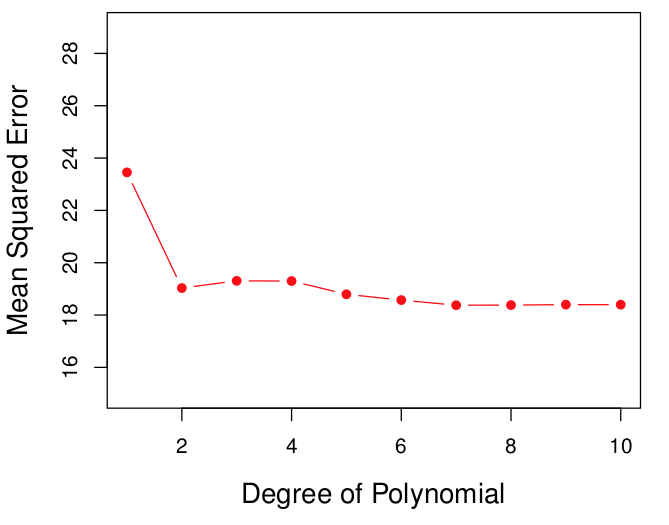
\includegraphics[width = \textwidth]{Fig5-2a}
\column{.45\textwidth}
\centering

Predicting $\texttt{mpg}$ using $\texttt{horsepower}$:
\begin{equation*}
	\texttt{mpg} = \beta_0 + \beta_1 \texttt{hp} + \beta_2 \texttt{hp}^2  + \cdots + \beta_p \texttt{hp} ^p
\end{equation*}
\InstructorList{
\item Shows the TEST error
\item Can conclude that linear isn't enough to model the data
}
\end{columns}

\end{frame}
%--- Next Frame ---%
\begin{frame}[c]{Rinse and repeat}

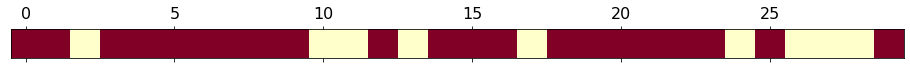
\includegraphics[width = \textwidth]{CV-subset0}
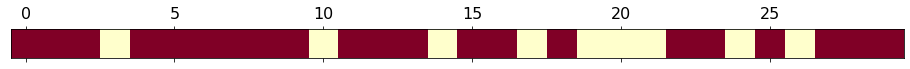
\includegraphics[width = \textwidth]{CV-subset1}
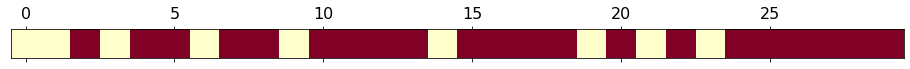
\includegraphics[width = \textwidth]{CV-subset2}
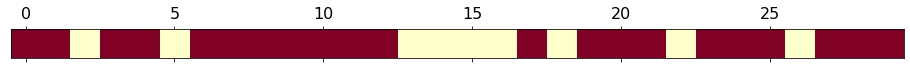
\includegraphics[width = \textwidth]{CV-subset3}
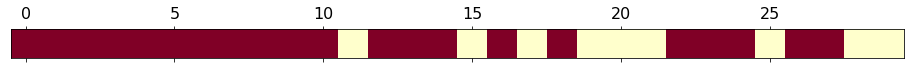
\includegraphics[width = \textwidth]{CV-subset4}
\begin{columns}
\column{.45\textwidth}
\centering

\column{.45\textwidth}
\centering

\end{columns}

\end{frame}
%--- Next Frame ---%
\begin{frame}[c]{Again example with \texttt{auto} data }

\begin{columns}
\column{.45\textwidth}
\centering
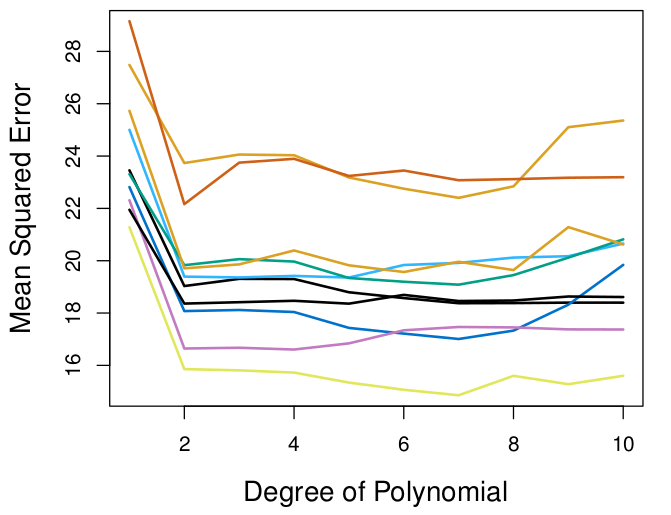
\includegraphics[width = \textwidth]{Fig5-2b}
\column{.45\textwidth}
\centering
\InstructorList{
\item Repeat the procedure with different splits
\item Highly variable results, no concensus about the error
\item Further complicated: Stats methods do worse when trained on fewer observations, so validation set error rate tends to overestimate test error rate when fitted on the whole data set.
}
\end{columns}

\end{frame}
%--- Next Frame ---%
{
  \setbeamercolor{background canvas}{bg=Apricot!25}
\begin{frame}[t]{Coding example in jupyter notebook}
\begin{columns}
\column{.45\textwidth}
\centering
\column{.45\textwidth}
\centering
\end{columns}
\end{frame}
}
%--- Next Frame ---%
%=====
\section{Leave-One-Out Cross-Validation (LOOCV)}
%=====
\begin{frame}[c]{The idea}
	\centering
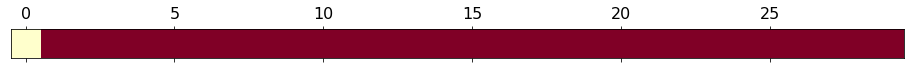
\includegraphics[width = \textwidth]{LOOCV-subset0.png}

\includegraphics[width = \textwidth]{LOOCV-subset1.png}

\includegraphics[width = \textwidth]{LOOCV-subset2.png}

\includegraphics[width = \textwidth]{LOOCV-subset3.png}

\includegraphics[width = \textwidth]{LOOCV-subset4.png}
$\vdots$

\includegraphics[width = \textwidth]{LOOCV-subset29.png}
\begin{columns}
\column{.45\textwidth}
\centering

\column{.45\textwidth}
\centering

\end{columns}

\end{frame}
%--- Next Frame ---%
\begin{frame}[c]{The idea in mathy words}

\begin{columns}
\column{.45\textwidth}
\centering
\begin{itemize}
	\item Remove $(x_1,y_1)$ for testing.
	\item Train the model on $n-1$ points: $\{(x_2,y_2), \cdots, (x_n,y_n)\}$
	\item Calculate $\mathrm{MSE}_1 = (y_1-\hat y_1)^2$
	\item[]
	\item Remove $(x_2,y_2)$ for testing.
	\item Train the model on $n-1$ points: $\{(x_1,y_1),(x_3,y_3), \cdots, (x_n,y_n)\}$
	\item Calculate $\mathrm{MSE}_2 = (y_2-\hat y_2)^2$
	\item []
	\item Rinse and repeat
\end{itemize}
\column{.45\textwidth}
\centering

Return the score:
\begin{equation*}
	CV_{(n)} = \frac{1}{n}\sum_{i=1}^n \mathrm{MSE}_i
\end{equation*}
\end{columns}

\end{frame}

%--- Next Frame ---%
\begin{frame}[t]{Again example with \texttt{auto} data}
	\begin{columns}
	\column{.45\textwidth}
	\centering
	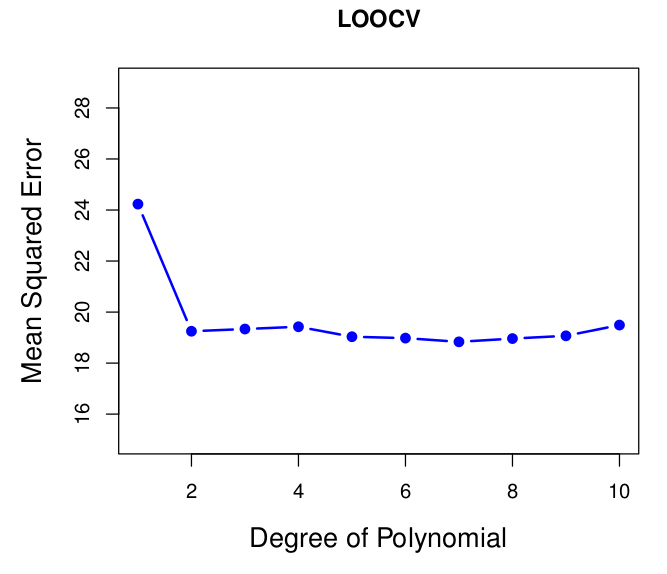
\includegraphics[align = c, width = \textwidth]{Fig5-4a}
	
	\column{.45\textwidth}
	\centering
	\InstructorList{
	  \item Point out that there is no randomness. Same every time. 
	}
	
	\end{columns}
	\end{frame}
%--- Next Frame ---%
{
  \setbeamercolor{background canvas}{bg=Apricot!25}
\begin{frame}[t]{Do the LOOCV coding section}
\begin{columns}
\column{.45\textwidth}
\centering
\column{.45\textwidth}
\centering
\end{columns}
\end{frame}
}
%--- Next Frame ---%
\begin{frame}[t]{LOOCV Pros and Cons}

\begin{columns}
\column{.45\textwidth}
\centering
\textbf{Advantages:}
\InstructorList{
\item Using almost all data every time
\item Stable results: no randomness so always the same answer on a fixed data set
\item Evaluation is performed with more testing data
}

\column{.45\textwidth}
\centering

\textbf{Disadvantages:}
\InstructorList{
\item Computationally expensive; fit the model $n$ times
\item Doesn't shake up the data enough: estimates from each fold are highly (positively) correlated so their averages have high variance.
}
\end{columns}
% \InstructorNotes{Next goal: Speed up the LOOCV, but to do that, we need to get some terminology first}
\end{frame}

%--- Next Frame ---%
% %=================
% \section{The one time you can cheat (by not computing every model fit)}
% %=================


% \begin{frame}[c]{Outliers}
% An \textit{outlier} is a point for which $y_i$ is far from the value predicted by the model.
% \InstructorNotes{$|y_i - \hat y_i|$ is large}
% \InstructorNotes{From Ch 3.3, stuff skipped earlier}

% \begin{columns}
% \column{.45\textwidth}
% \centering

% 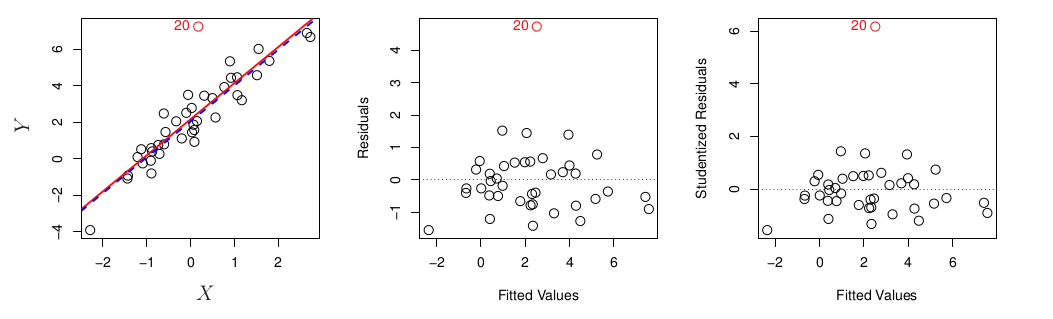
\includegraphics[width = \textwidth, align = c, trim = 0 0 670 0, clip]{Fig3-12}
% \column{.45\textwidth}
% \centering
% \InstructorList{
% \item Red line: Regression with all data
% \item Blue dashed: Regression after removing outlier 20
% \item Point out that even though this is an outlier, didn't have much effect in this case.
% }
% \end{columns}


% \end{frame}
% %--- Next Frame ---%
% \begin{frame}[t]{Residuals}

% 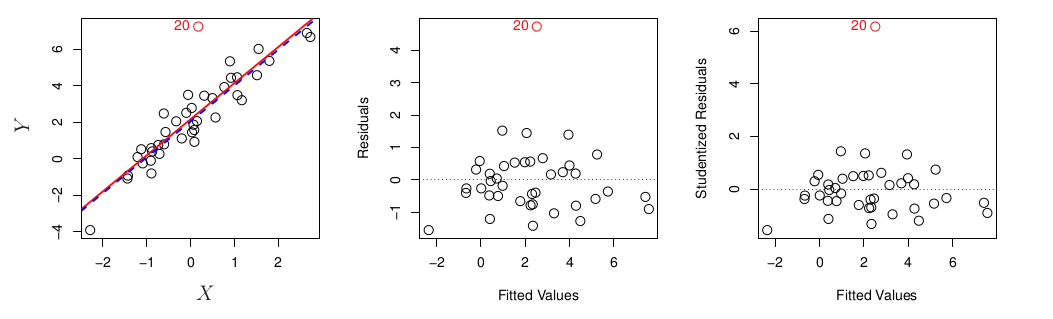
\includegraphics[width = \textwidth, align = c, trim = 0 0 0 0, clip]{Fig3-12}
% \begin{columns}
% \column{.45\textwidth}
% \centering
% \InstructorNotes{
% Residuals are $|y_i-\hat y_i|$.  Problem with no clear way to decide which is far enough to constitute outlier. Studentized version divides by std error of the points. Common choice is $\geq 3$ is outlier.
% }
% \column{.45\textwidth}
% \centering

% \end{columns}

% \end{frame}
% %--- Next Frame ---%
% \begin{frame}[t]{High Leverage}

% \begin{columns}
% \column{.45\textwidth}
% \centering
% 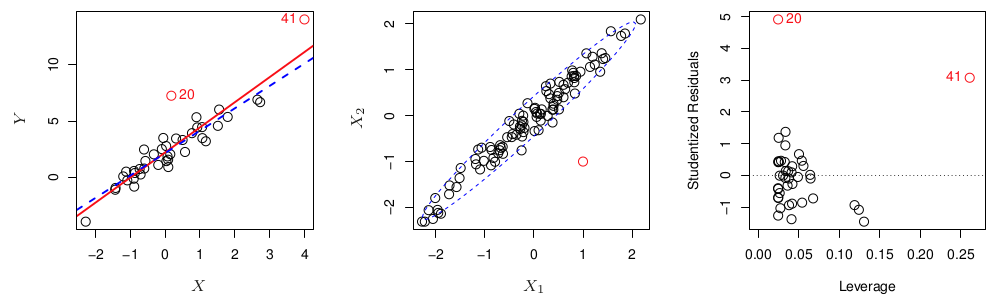
\includegraphics[width = \textwidth, trim = 0 0 670 0, clip]{Fig3-13}

% \column{.45\textwidth}
% \centering

% Observations with \textit{high leverage} have an unusual value for $x_i$.
% \InstructorList{
% \item Same data as previous but with extra data point 41
% \item Easy to find in $p=1$ case, as at left, since just look for big x value.
% \item Red line: fit all data
% \item Blue dashed line: fit after removing high leverage point 41
% \item Point out big movement in linear regression line
% }
% \end{columns}

% \end{frame}
% %--- Next Frame ---%
% \begin{frame}[t]{Leverage statistic}

% \begin{columns}
% \column{.3\textwidth}
% \centering

% 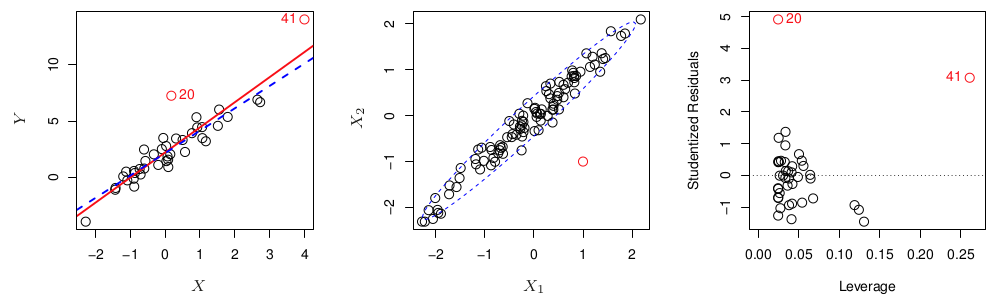
\includegraphics[width = \textwidth, trim = 0 0 670 0 , clip]{Fig3-13}
% \column{.3\textwidth}
% \centering

% 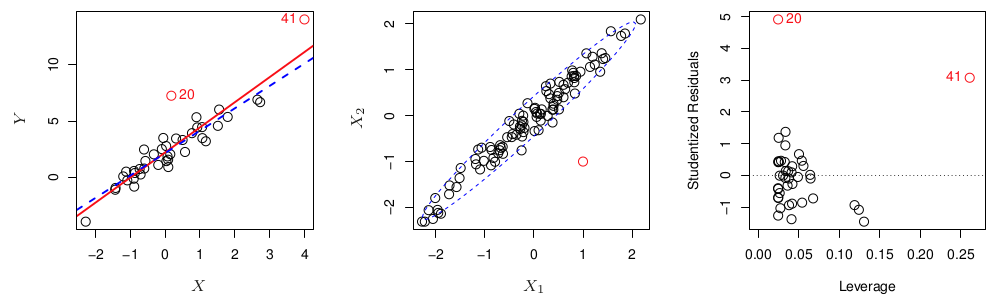
\includegraphics[width = \textwidth, trim = 670 0 0 0 , clip]{Fig3-13}
% \column{.3\textwidth}
% \centering
% Version for $p=1$
% \begin{equation*}
% 	h_i = \frac{1}{n} + \frac{(x_i - \overline x)^2}{\sum_{j=1}^n (x_j - \overline x)^2}
% \end{equation*}
% \InstructorNotes{Generalizes to higher $p$, but not defined here. Compy can do it.}


% \end{columns}
% \end{frame}
% %--- Next Frame ---%
% \begin{frame}[t]{Leverage statistic properties}

% \begin{columns}
% \column{.45\textwidth}
% \centering
% \begin{equation*}
% 	h_i = \frac{1}{n} + \frac{(x_i - \overline x)^2}{\sum_{j=1}^n (x_j - \overline x)^2}
% \end{equation*}
% \column{.45\textwidth}
% \centering

% \InstructorList{
% \item Increases with distance of $x_i$ from $\overline x$.
% \item Always between $1/n$ and 1
% \item Average leverage for all observations is always $(p+1)/n$ (previous page this is $2/41 = 0.049$)
% \item If leverage stat is way bigger than $(p+1)/n$, then likely high leverage.
% \item 41 on previous page is both high leverage and outlier, so bad all around
% \item 20 on previous page had little effect on linear regression because low leverage even though it's an outlier
% }
% \end{columns}

% \end{frame}
% %--- Next Frame ---%
% \begin{frame}[t]{Speeding up LOOCV}

% 	{\color{red}Warning:} This only works for least squares linear or polynomial regression.

% 	\bvfill
% 	\begin{equation*}
% 		\frac{1}{n}\sum_{i=1}^n \mathrm{MSE}_i = CV_{(n)} = \frac{1}{n}\sum_{i=1}^n \left( \frac{y_i - \hat y_i}{1-h_i} \right)^2
% 	\end{equation*}

% 	\bvfill
% \begin{columns}
% \column{.45\textwidth}
% \centering
% \InstructorList{
% \item Left side is original LOOCV computation
% \item Right side uses $\hat y_i$ fit on the whole data set
% }

% \column{.45\textwidth}
% \centering
% \InstructorList{
% \item Yay, only one model fitting!
% \item Looks similar to regular MSE
% }
% \end{columns}

% \end{frame}
%--- Next Frame ---%
\begin{frame}[c]{TL;DR}

\vspace{1in}

\begin{columns}
	\column{.3\textwidth}
	\centering
	\textbf{Validation set}
	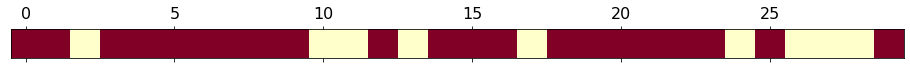
\includegraphics[width = \textwidth]{CV-subset0}
	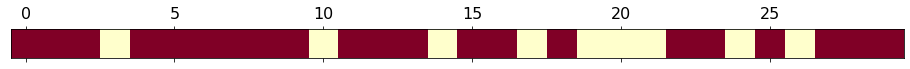
\includegraphics[width = \textwidth]{CV-subset1}
	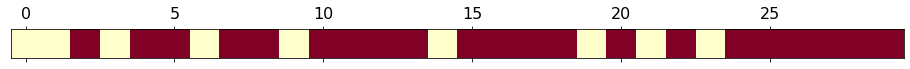
\includegraphics[width = \textwidth]{CV-subset2}
	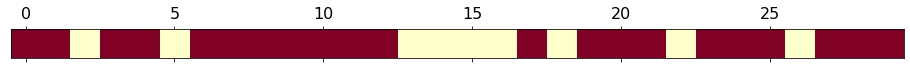
\includegraphics[width = \textwidth]{CV-subset3}
	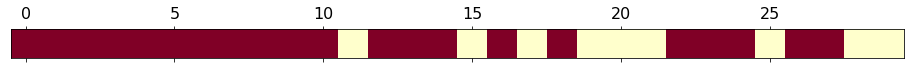
\includegraphics[width = \textwidth]{CV-subset4}
\column{.3\textwidth}
\centering
\textbf{LOO-CV}
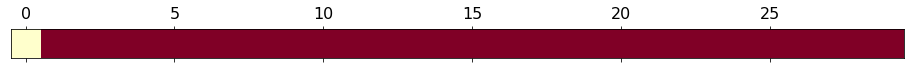
\includegraphics[width = \textwidth]{LOOCV-subset0.png}

\includegraphics[width = \textwidth]{LOOCV-subset1.png}

\includegraphics[width = \textwidth]{LOOCV-subset2.png}
% 
\includegraphics[width = \textwidth]{LOOCV-subset3.png}
% 
\includegraphics[width = \textwidth]{LOOCV-subset4.png}
$\vdots$

\includegraphics[width = \textwidth]{LOOCV-subset29.png}

\column{.35\textwidth}
\centering
\textbf{LOO-CV Score}
\begin{equation*}
	CV_{(n)} = \frac{1}{n}\sum_{i=1}^n \mathrm{MSE}_i
\end{equation*}

% \textbf{Cheap trick for regression}
% \begin{equation*}
% 	 CV_{(n)} = \frac{1}{n}\sum_{i=1}^n \left( \frac{y_i - \hat y_i}{1-h_i} \right)^2
% \end{equation*}
\end{columns}


\end{frame}
%--- Next Frame ---%
% %----------------
\begin{frame}[t]{Next time}

	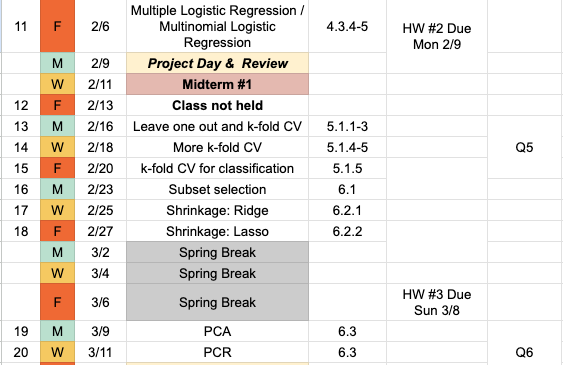
\includegraphics[align = c, width = .65\textwidth]{Schedule-S26-Lecs11_to_20}
	
\end{frame}
%--- Next Frame ---%


\end{document}
